\documentclass[a4paper,10pt,oneside]{article}
\usepackage[polutonikogreek,italian]{babel}
\usepackage[utf8x]{inputenc}
\usepackage{amsmath}
\usepackage{amsthm}
\usepackage{amssymb}
\usepackage{amscd}
\usepackage{graphicx}
\usepackage{float}
\usepackage{array}
\usepackage{rotating}
\usepackage[small]{caption}
\usepackage{lscape}
\usepackage{fancybox}
\usepackage{booktabs}
\usepackage[noanswer]{exercise}
\parindent0ex
\renewcommand{\fboxsep}{0.4cm}
\usepackage{hyperref}
\renewcommand{\textfraction}{0.05}
\renewcommand{\topfraction}{0.95}
\renewcommand{\bottomfraction}{0.95}
\renewcommand{\floatpagefraction}{0.35}
\renewcommand{\ExerciseName}{Esercizio}
\renewcommand{\ExerciseListName}{Es}
\setcounter{totalnumber}{5}
\restylefloat{figure}
\begin{document}
\thispagestyle{empty}
 \section*{Le forze}
\vspace{1cm}

\section*{Natura vettoriale delle forze}

Un utile esercizio per  dimostrare la natura vettoriale consiste nel costruire il semplice sistema illustrato in figura  [\ref{fig:natura_forze}]. Quando avremo terminato l'allestimento del sistema la massa centrale e le masse laterali saranno immobili. Sulla $M_1$ agirà la forza $\mathbf{F}_1=M_1\mathbf{g}$, sulla massa $M_2$ la forza $\mathbf{F}_2=M_2\mathbf{g}$ e sulla massa $M_3$ la forza $\mathbf{F}_3=M_3\mathbf{g}$. Siccome le masse sono immobili e il laboratorio, al fine dell'analisi di questo esperimento può essere considerato un sistema di riferimento inerziale, sulle masse oltre alla forza di gravità dovranno agire delle forze atte a neutralizzare i pesi.

\begin{figure}[H]
 \centering
 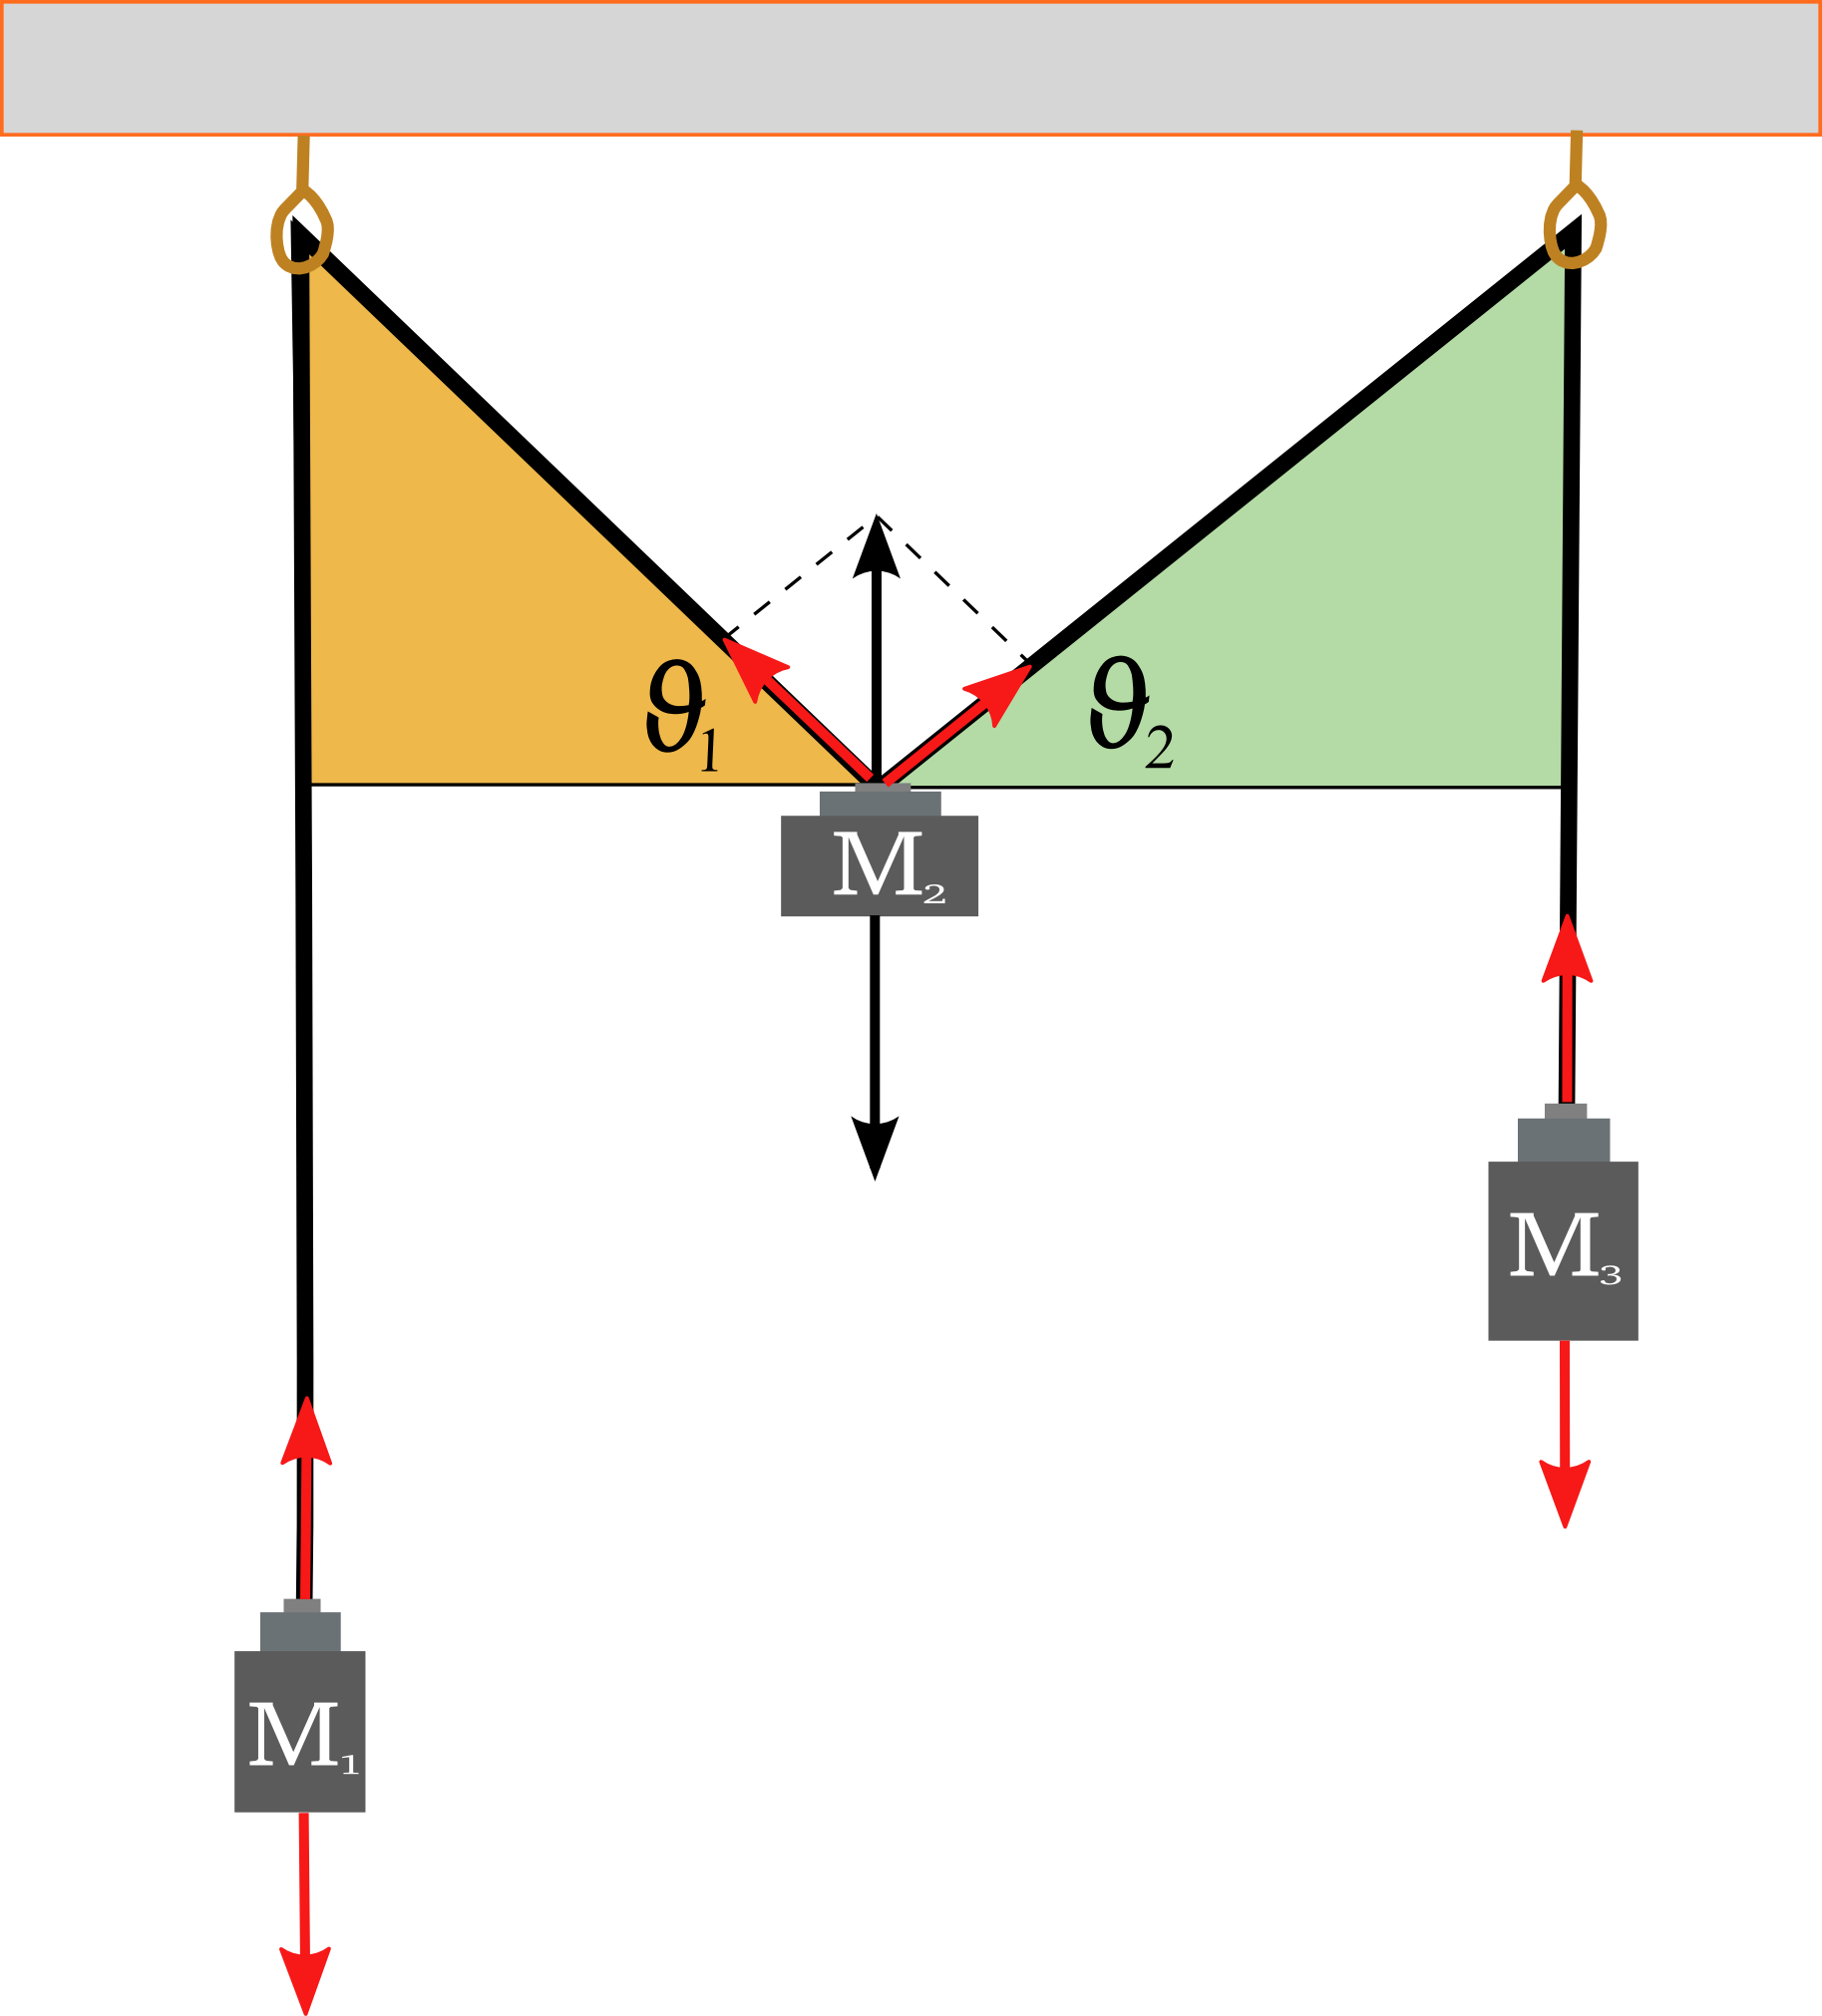
\includegraphics[width=0.8\textwidth]{../immagini/natura_vettoriale_forze1.png}
 % natura_vettoriale_forze1.png: 1846x2042 pixel, 300dpi, 15.63x17.29 cm, bb=0 0 443 490
 \caption{La massa al centro è immobile, la somma vettoriale delle forze esercitate dalle due masse poste ai lati deve uguagliare il peso della massa centrale}
 \label{fig:natura_forze}
\end{figure}

 Analizziamo la situazione della massa centrale, su di essa agiranno  la forza $\mathbf{F}_2$ dovuta alla massa $M_2$ e le forze $F_1$ ed $F_3$ dovute alle masse laterali. Scriviamo le componenti delle forze applicate alla massa centrale:

\begin{equation}
 \mathbf{F}_2=(0,-M_2g)
\end{equation}

le forze dovute alle masse laterali sono invece:
\begin{equation}
 \mathbf{F}_{21}=(-F_1\cos \theta_1,F_1\sin\theta_1)
\end{equation}
\begin{equation}
 \mathbf{F}_{23}=(F_3\cos\theta_2,F_3\sin\theta_2)
\end{equation}
dove con $\mathbf{F}_{21}$ abbiamo indicato la forza esercitata dalla $M_1$ sulla massa $M_2$ e con $\mathbf{F}_{23}$ la forza esercitata dalla massa $M_3$ sulla massa $M_2$.

Se le forze si comportano come dei vettori per raggiungere l'equilibrio dovremo ottenere:

\begin{equation}\label{eq:eq_forze}
  \mathbf{F}_2+\mathbf{F}_{21}+\mathbf{F}_{23}=0
\end{equation}

l'equazione [\ref{eq:eq_forze}] ci dice quindi che:
\begin{equation}\label{eq:forze_x}
 -F_1\cos \theta_1+F_3\cos\theta_2=0
\end{equation}
ovvero la somma delle forze esercitate delle masse esterne deve avere una componente orizzontale nulla e che:
\begin{equation}\label{eq:forze_y}
 F_3\sin\theta_2+F_1\sin\theta_1=M_2g
\end{equation}
ovvero la somma delle componenti verticali deve avere lo stesso modulo e la stessa direzione della forza peso agente sulla massa centrale ma verso opposto.
In classe\footnote{Come è stato fatto durante la lezione di sabato 5 febbraio 2011} possiamo verificare che entro i limiti sperimentali impostici dalle attrezzature le equazioni [\ref{eq:forze_x}] e [\ref{eq:forze_y}] sono verificate. I passi da seguire per effettuare la misura sono:
\begin{itemize}
 \item Usando una bilancia a bracci misuriamo le masse $M_1$, $M_2$ ed $M_3$
 \item Usando un righello misuriamo i cateti dei due triangoli rettangoli formati dal sistema di tre masse
\item Tramite la relazione trigonometrica $\tan\theta=<\mathrm{cateto\ opposto}>/<\mathrm{cateto\ adiacente}>$ ricaviamo il seno ed il coseno dell'angolo.
\end{itemize}




\section*{Moto di masse collegate da una corda inestensibile}

L'analisi del moto di due masse collegate da un filo inestensibile verrà svolta in due momenti, per prima cosa analizzeremo il caso statico, ovvero le due masse sono immobili rispetto al sistema di riferimento del laboratorio, successivamente elimineremo il vincolo di staticità e lasceremo che le due masse si muovano sotto la spinta della gravità. Nella nostra analisi ignoreremo:
\begin{itemize}
 \item L'attrito viscoso esercitato dall'aria durante il moto delle masse
 \item Il momento di inerzia della carrucola su cui scorre il filo
 \item La massa del filo di collegamento
 \item Le deformazioni elastiche del filo di collegamento e delle masse
\end{itemize}


\subsection*{Caso statico}
Nel caso statico la massa sospesa al filo e il carrello posto sulla guidovia a cuscino d'aria sono immobili, pertanto la somma totale delle forze agenti deve essere nulla. Sul carico sospeso agiranno la forza di gravità:

\begin{equation}
 \mathbf{F}=M_1\mathbf{g}
\end{equation}

dove $\mathbf{g}=-g\hat{\mathbf{y}}$ è il vettore accelerazione di gravità, ed una forza uguale in modulo e direzione ed opposta in verso esercitata dal sensore di forza tramite il filo ed il carrello:

\begin{equation}
 \mathbf{F_c}=-M_1\mathbf{g}=-\mathbf{F}
\end{equation}

come risultato avremo che la forza indicata dal nostro sensore sarà in modulo pari alla forza peso agente sulla massa $M_1$.

\begin{figure}[H]
 \centering
 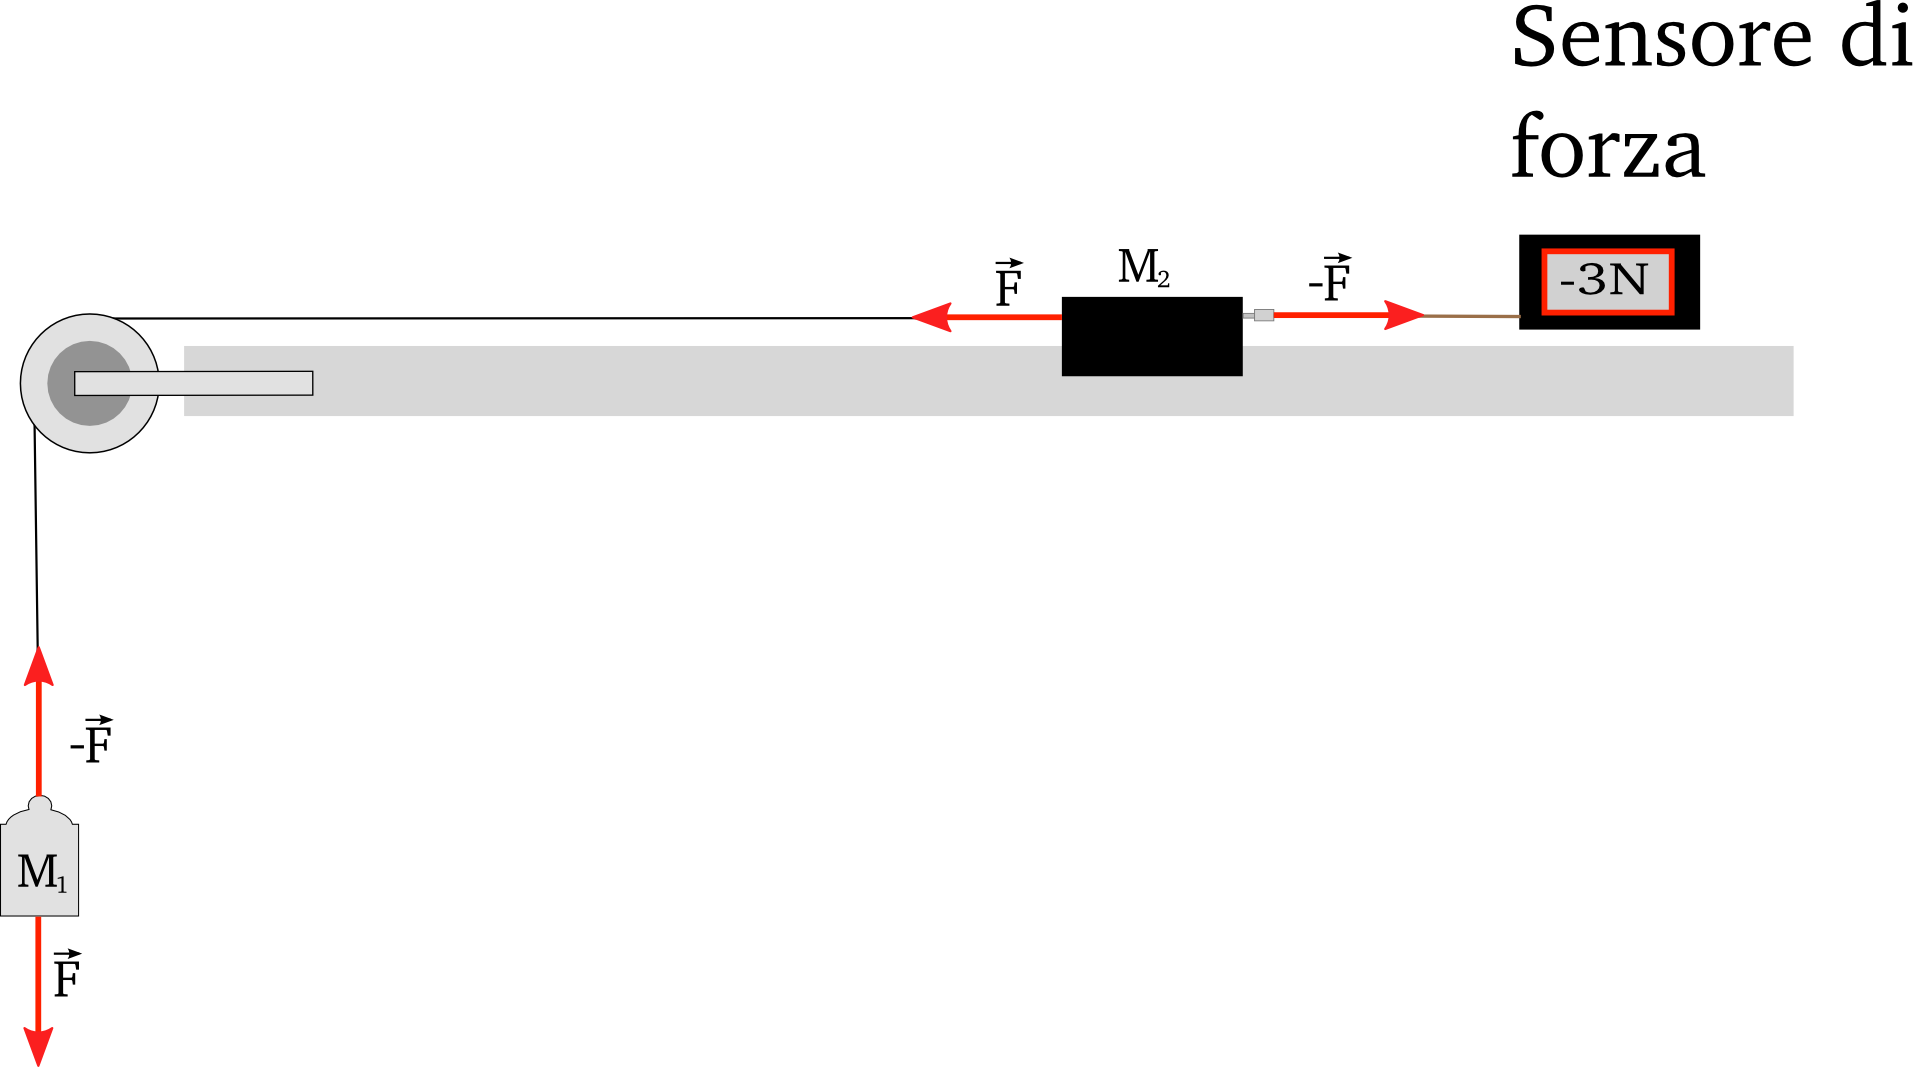
\includegraphics[width=\textwidth]{../immagini/masse_filo_statico.png}
 % masse_filo_statico.png: 1914x1067 pixel, 200dpi, 24.31x13.55 cm, bb=0 0 689 384
 \caption{Due masse sono collegate tra loro da una fune, il sistema è statico}
 \label{fig:filo_statico}
\end{figure}

\subsection*{Caso dinamico}

Nel caso dinamico il carrello ed il carico sospeso si stanno muovendo con una certa accelerazione $\mathbf{a}$. Come possiamo calcolare il modulo di $\mathbf{a}$?
Per prima cosa notiamo che la forza responsabile del moto delle due masse è unicamente la forza di gravità applicata alla massa sospesa:
\begin{equation}
 \mathbf{F}_g=M_1\mathbf{g}
\end{equation}
questa forza non è applicata unicamente alla massa che sta cadendo, tramite il filo inestensibile è applicata anche alla massa che sta scivolando (quasi) senza attrito sul cuscino d'aria generato dalla guidovia. La seconda legge di Newton ci dice quindi:
\begin{equation}\label{eq:filo_dinamico}
 \mathbf{F}=M_1\mathbf{g}=(M_1+M_2)\mathbf{a}
\end{equation}

l'equazione [\ref{eq:filo_dinamico}] ci permette quindi di ricavare il valore del modulo dell'accelerazione:
\begin{equation}\label{eq:filo_dinamico_res}
 |\mathbf{a}|=\frac{M_1}{M_1+M_2}g
\end{equation}
il risulato [\ref{eq:filo_dinamico_res}] è in accordo con i dati che possiamo raccogliere in laboratorio ed anche con il senso comune, l'accelerazione della massa legata è infatti più piccola di quella che questa avrebbe nel caso cadesse senza alcun collegamento con la massa posta sulla guidovia. Notiamo che a causa della inestensibilità del filo la velocità e l'accelerazione della massa in caduta e di quella in fase di scorrimento devono essere uguali.

\begin{figure}[H]
 \centering
 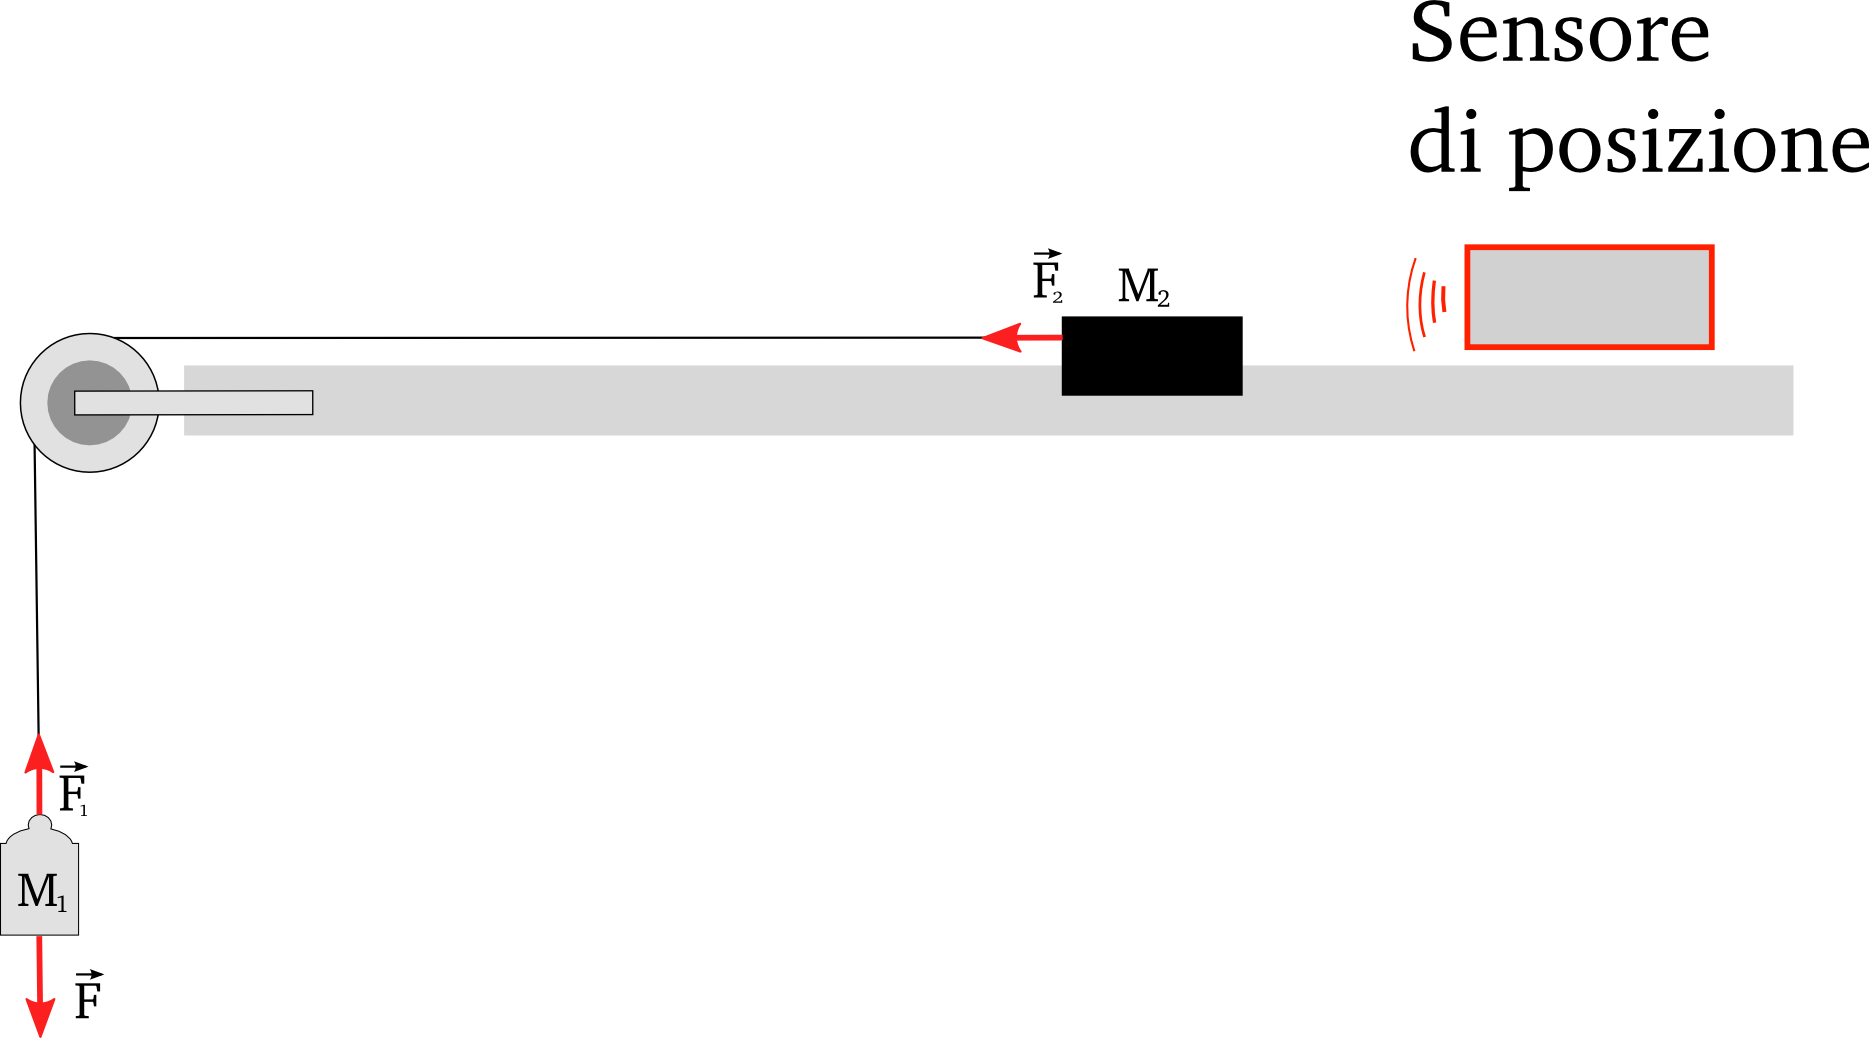
\includegraphics[width=\textwidth]{../immagini/masse_filo_dinamico.png}
 % masse_filo_dinamico.png: 1869x1038 pixel, 200dpi, 23.74x13.19 cm, bb=
 \caption{Due masse sono collegate da una corda inestensibile e si stanno muovendo verso il basso sotto l'effetto della forza di gravità}
 \label{fig:filo_dinamico}
\end{figure}





\section*{Forze fittizie}

La seconda legge di Newton
\begin{equation}\label{eq:newton_2}
 \mathbf{F}=m\mathbf{a}_I
\end{equation}
come è noto è applicabile unicamente se l'accelerazione è misurata rispetto ad un sistema di riferimento inerziale\footnote{Per sistema inerziale considereremo d'ora innanzi un sistema che si muove di moto rettilineo uniforme rispetto alle stelle fisse}. L'equazione [\ref{eq:newton_2}] non è quindi utilizzabile per delle misure effettuate in un laboratorio solidale con la terra o un qualsiasi altro sistema di riferimento in moto accelerato rispetto alla stelle fisse. Per ottenere un'equazione applicabile da un osservatore in un sistema accelerato, scriviamo l'accelerazione misurata da un osservatore inerziale come somma dell'accelerazione del sistema di riferimento non inerziale (misurata dall'osservatore inerziale) e dell'accelerazione misurata dall'osservatore non inerziale:
\begin{equation}
 \mathbf{a}_I=\mathbf{a}_0+\mathbf{a}
\end{equation}
dove $\mathbf{a}_I$ è l'accelerazione misurata dall'osservatore inerziale, $\mathbf{a_0}$ è l'accelerazione del sistema non inerziale misurata dall'osservatore inerziale e $\mathbf{a}$ è l'accelerazione misurata dall'osservatore solidale con il sistema non inerziale.
Questa definizione ci permette di riscrivere l'equazione [\ref{eq:newton_2}] come:
\begin{equation}
 \mathbf{F}=m\mathbf{a}_0+m\mathbf{a}
\end{equation}
ovvero introducendo la forza $\mathbf{F}_0$
\begin{equation}\label{eq:fittizia_2}
 \mathbf{F}+\mathbf{F}_0=m\mathbf{a}
\end{equation}
dove:
\begin{equation}\label{eq:forza_fittizia}
 \mathbf{F}_0=-m\mathbf{a}_0
\end{equation}
e rappresenta la forza fittizia che un osservatore non inerziale deve introdurre per giustificare le osservazioni fatte all'interno del suo sistema di riferimento.

\subsection*{L'accelerometro}
Immaginiamo di realizzare un sistema simile a quello schematizzato in figura [\ref{fig:accelerometro}] che consiste di un contenitore, di una molla  e di una piccola massa $m$. Considereremo la molla priva di massa e nullo l'attrito tra la massa $m$ e il fondo del contenitore. Inoltre il sistema molla-massa sarà vincolato ad una sponda della scatola. Sappiamo che la forza esercitata da una molla ideale\footnote{Legge di Hooke} è:
\begin{equation}
 \mathbf{F}=-K\mathbf{x}
\end{equation}
dove $K$\footnote{Costante elastica} è una costante che dipende dal tipo di molla utilizzata ed $x$ è un vettore che ci indica di quanto la molla si è spostata rispetto al suo punto di equilibrio. Lo strumento che abbiamo ora introdotto è grado di indicarci quanto vale l'accelerazione di una automobile?

\begin{figure}[H]
 \centering
 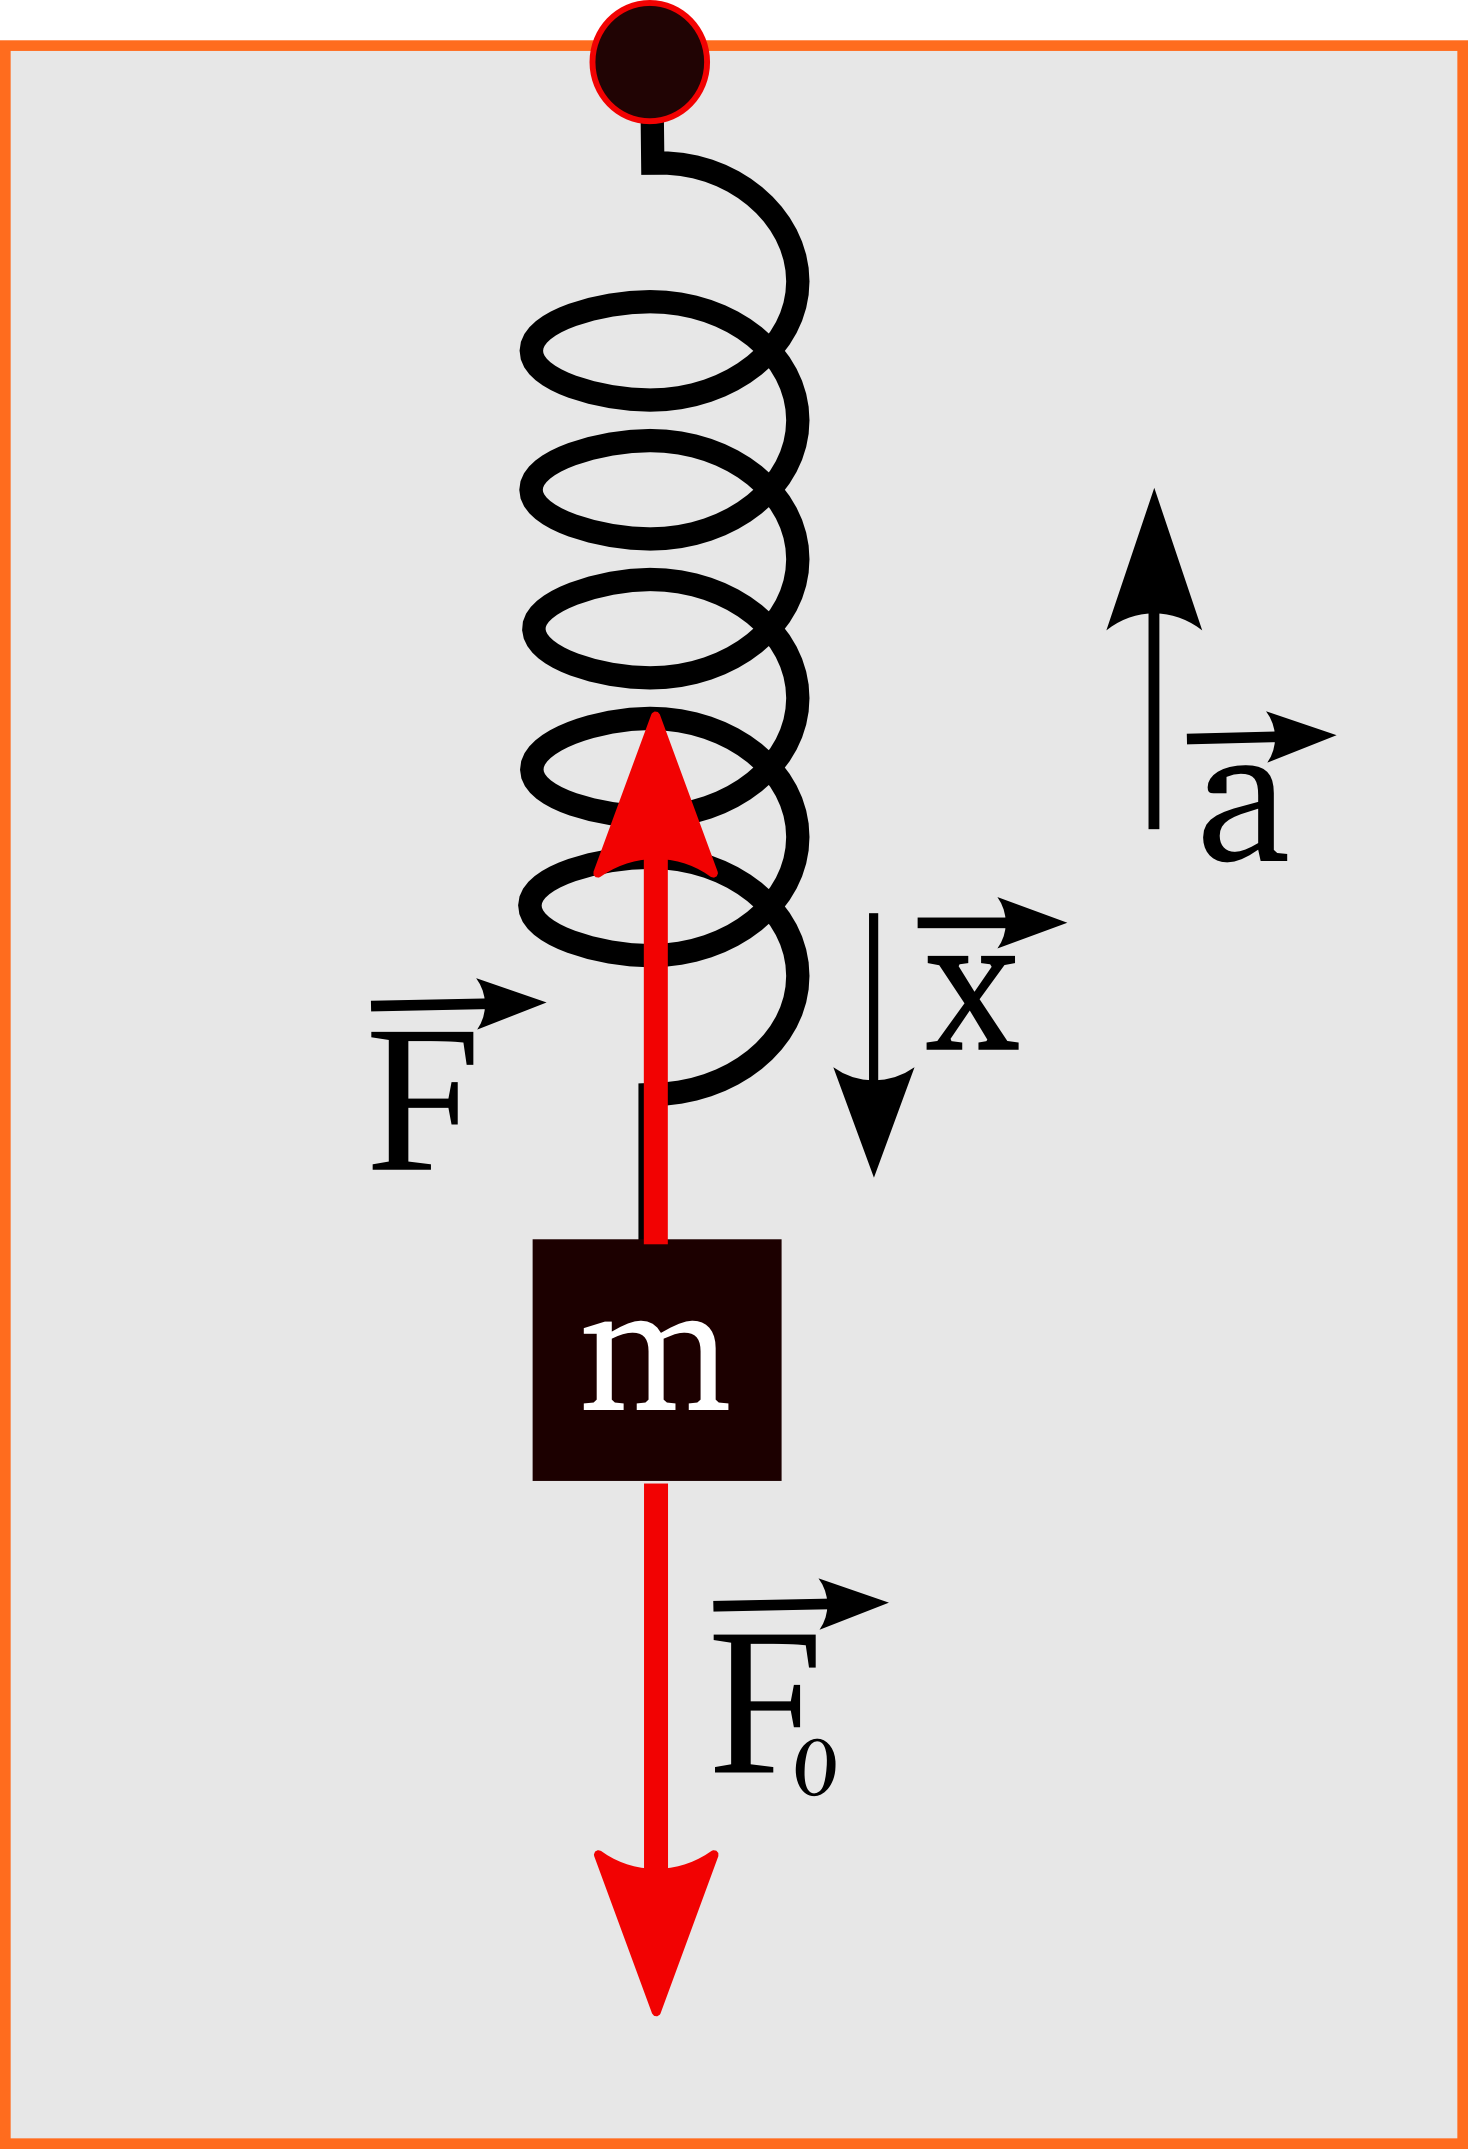
\includegraphics[height=0.4\textheight]{../immagini/accelerometro.png}
 % accelerometro.png: 1545x2186 pixel, 1200dpi, 3.27x4.63 cm, bb=
\caption{L'insieme molla e massa si trova all'interno di un contenitore privo di attrito e disposto orizzontalmente sul cruscotto di una automobile}
 \label{fig:accelerometro}
\end{figure}

Per rispondere a questo quesito supponiamo che un automobilista posizioni il nostro accelerometro orizzontalmente sopra il cruscotto della sua auto, incollandolo di modo che non si possa muovere. Un osservatore inerziale che vede la macchina accelerare con una certa accelerazione $\mathbf{a}_I$ dedurrà che sulla massa $m$ collegata alla molla, e ferma rispetto alla macchina, agirà una forza $m\mathbf{a}_I$ e scriverà quindi la seconda legge di Newton come:
\begin{equation}
 \mathbf{F}=m\mathbf{a}_I
\end{equation}
lo stesso osservatore è in grado inoltre di capire che la forza che fa accelerare la massa collegata alla molla è esercitata dalla molla stessa, conoscendo quindi la legge delle molle riesce a scrivere:
\begin{equation}
 -K\mathbf{x}=m\mathbf{a}_I
\end{equation}
Chiaramente anche l'osservatore non inerziale seduto all'interno dell'automobile vedrà la molla allungarsi, al fine di esercitare sulla massa $m$ una certa forza, l'osservatore non inerziale misurerà però una accelerazione nulla dato che rispetto al suo sistema di riferimento la molla non si sta muovendo\footnote{Se l'accelerazione è costante}, l'osservatore non inerziale applicherà quindi l'equazione [\ref{eq:fittizia_2}] ricavando:
\begin{equation}
 \mathbf{F}+\mathbf{F_0}=0
\end{equation}
per giustificare le sue osservazioni l'osservatore non inerziale dovrà presupporre la presenza di una forza \emph{fittizia} $\mathbf{F}_0$ nel suo sistema di riferimento responsabile dell'allungamento della molla.
L'entità di tale forza sarà:
\begin{equation}\label{eq:accel_1}
 \mathbf{F_0}=K\mathbf{x}
\end{equation}
dall'equazione [\ref{eq:accel_1}] e dalla [\ref{eq:forza_fittizia}] possiamo ricavare l'accelerazione (in modulo) del sistema non inerziale:
\begin{equation}\label{eq:accel_2}
a_0=-\frac{Kx}{m}
\end{equation}


\subsection*{Il bicchiere}


Cosa succede se applichiamo una forza costante ad un contenitore al cui interno abbiamo posto dell'acqua colorata? Un osservatore inerziale noterà che la superficie dell'acqua prima parallela al terreno (e quindi perpendicolare alla direzione dell'accelerazione di gravità) forma un certo angolo con l'orizzontale dipendente dall'accelerazione del contenitore. Un osservatore non inerziale posto all'interno del vaso vedrebbe inclinarsi la sua linea di orizzonte rispetto alle pareti del vaso stesso e dovrebbe supporre l'insorgere di una forza fittizia che interpreterebbe come un aumento del suo peso. 
\begin{figure}[H]
 \centering
 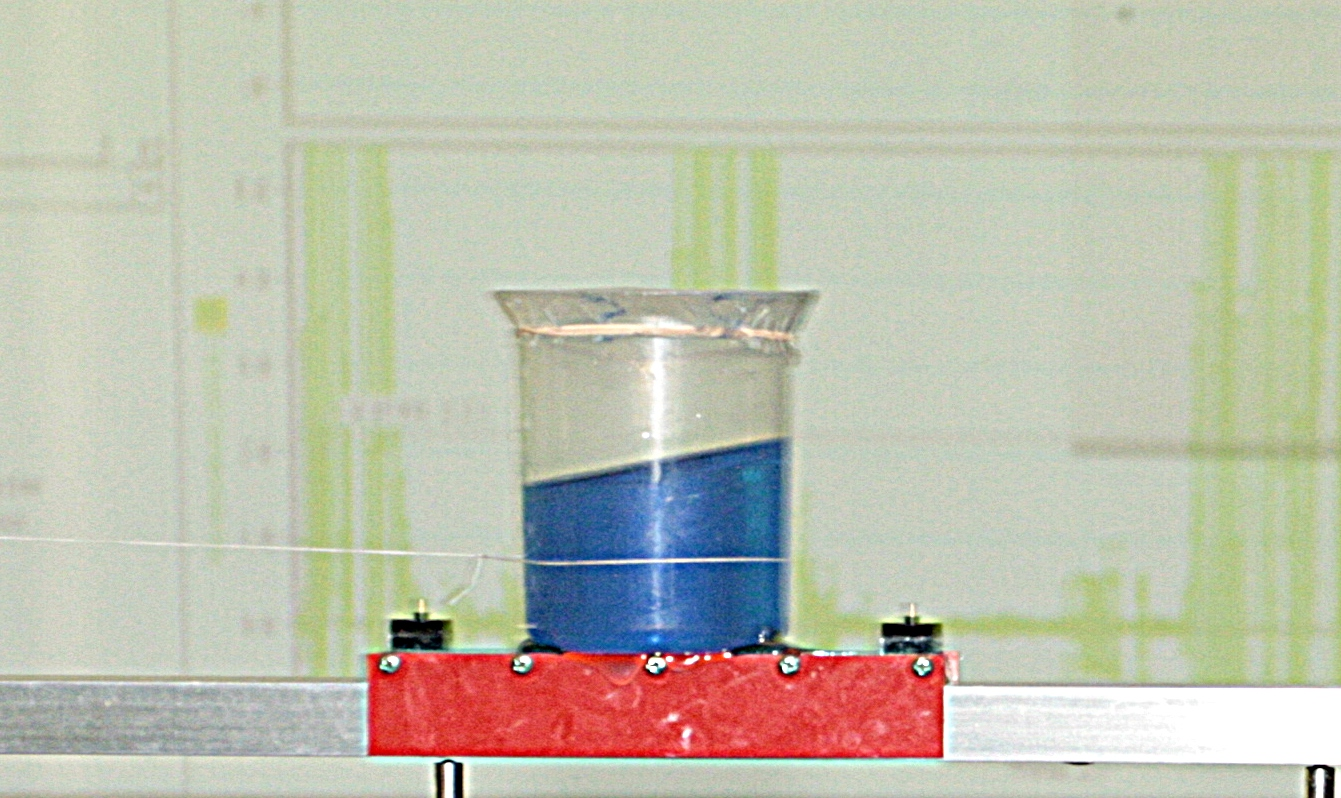
\includegraphics[width=0.8\textwidth]{../immagini/vasetto.jpg}
 % vasetto.jpg: 1341x798 pixel, 72dpi, 47.31x28.15 cm, bb=0 0 1341 798
 \caption{Quando il beker contenente dell'acqua colorata viene accelerato si ha una inclinazione della superficie libera del liquido}
 \label{fig:vasetto_accelerato}
\end{figure}
Come possiamo vedere dalla figura [\ref{fig:vasetto_rappresentazione}] il pelo libero dell'acqua forma un angolo $\theta$ con l'orizzontale del laboratorio, misurando tale angolo nella fotografia ripresa durante l'esercitazione, possiamo calcolare il valore dell'accelerazione  del vasetto. Tramite la definizione geometrica di tangente:
\begin{equation}
 \tan\theta=\frac{\textrm{cateto\ opposto}}{\textrm{cateto\ adiacente}}
\end{equation}
e osservando che il cateto opposto nell'immagine rappresenta il modulo del vettore accelerazione incognito, possiamo ricavare la relazione:
\begin{equation}
|\mathbf{a_0}|=g\tan\theta
\end{equation}



\begin{figure}[H]
 \centering
 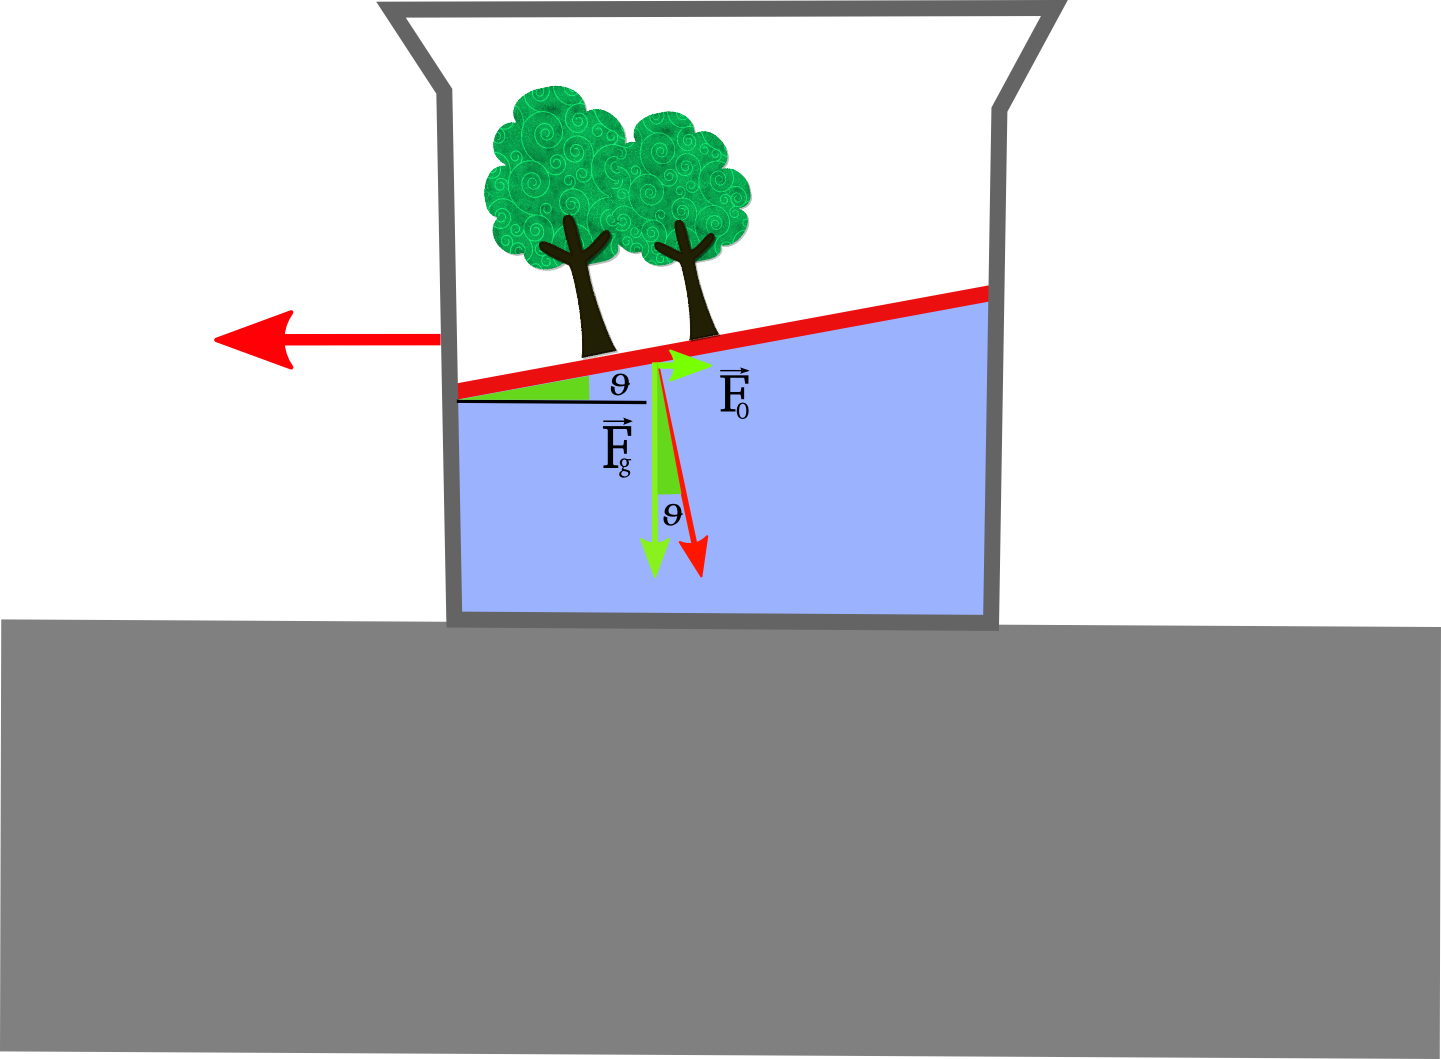
\includegraphics[width=0.8\textwidth]{../immagini/vasetto_disegno.png}
 % vasetto_disegno.png: 1921x1412 pixel, 400dpi, 12.20x8.97 cm, bb=
\caption{Per un osservatore solidale con il vasetto la forza di gravità sembra aumentare e la linea di orizzente si inclina rispetto alla pareti del vasetto} \label{fig:vasetto_rappresentazione}
\end{figure}



\end{document}
